The observation of the NS merger GW170817 has provided for the first time the empirical
estimate of the tidal deformation of NS induced by strong gravitational field between 
the two companions of a merging binary pulsar \citep{hinderer2008tidal,hinderer2010tidal}. 
In this chapter, 
we discuss briefly, within the frame of General Relativity, how a static spherical NS can be
tidally deformed by gravitation, gaining nonzero gravito-multipole moments which are
directly proportional to the strength of gravitation \citep{damour2009relativistic}.
The tidal deformation moments of different multipoles are determined in the present work 
with the mean-field based EoS of spin-polarized NS matter using the explicit expressions 
of the Love numbers given by GR \citep{perot2021role}. The obtained results for the tidal
deformability as well as the gravitational mass $M$ and radius $R$ of \gls{NS} are 
compared in details with the astrophysical constraints deduced from the observation 
of GW170817.

\subsection{Einstein equations of relativistic neutron star}%
\label{sec3.1}
In general, the line element of metric in the static isotropic spacetime can be 
expressed within GR  \citep{oppenheimer1939massive} in terms of spatial spherical 
coordinates as
\begin{equation}
        ds^2 = g_{\mu\nu}dx^\mu dx^\nu= - e^{2\nu(r)}c^2dt^2 + e^{2\lambda(r)}dr^2 + 
				r^2 d\theta^2 + r^2\sin^2\theta d\phi^2, \label{metr}
\end{equation}
where arbitrary functions $\nu(r)$ and $\lambda(r)$ are determined locally by the
mass-energy density within the sphere of radius $r$. In the vicinity of a 
static spherical NS, the spacetime geometry is determined from the pressure and 
mass-energy density of NS matter (treated as a perfect fluid), and the  
energy-momentum tensor is obtained in \gls{GR} as
\begin{equation}
        T^{\mu\nu}= Pg^{\mu\nu} + \left( \frac{P}{c^2} +\rho \right) u^\mu u^\nu,\quad
				g_{\mu\nu}u^\mu u^\nu=u_\nu u_\nu=-c^2.
\end{equation}
Here $P$ and $\rho$ are the pressure and mass-energy density of NS matter, respectively,
$u^\mu = dx^\mu/d\tau$ is the local fluid 4-velocity. The Einstein's field 
equations of neutron star are written as 
\begin{equation}
        G^{\mu\nu} = \frac{8\pi G}{c^4} T^{\mu\nu}. \label{Ein} 
\end{equation}
Keeping the nonrelativistic limit to the static Newtonian gravitation, the 
Einstein's field equations (\ref{Ein}) can be reduced to the following differential 
equations which are known as Tolman-Oppenheimer-Volkoff (\gls{TOV}) equations 
\citep{oppenheimer1939massive}
\begin{eqnarray}
\frac{d P(r)}{dr}&=& -\frac{G \rho(r)\mathcal{M}(r)}{c^2 r^2} 
 \left[ 1+\frac{P(r)}{\rho(r)}\right] 
\left[1+\frac{4 \pi P(r) r^3}{c^2 \mathcal{M}(r)} \right] 
\left[ 1-\frac{2G \mathcal{M}(r)}{c^2 r} \right]^{-1}, \nonumber \\
d\mathcal{M}(r) &=& 4\pi r^2 \rho(r)dr, \label{tov} 
\end{eqnarray}
where $r$ is the radial coordinate in Schwarzschild metric (\ref{metr}), and 
$\mathcal{M}(r)$ is the gravitational mass enclosed within sphere of radius $r$. 
$\rho(r)$ and $P(r)$ are the mass-energy density and pressure of NS matter at 
distance $r$ from the star center, respectively. The \gls{TOV} equations (\ref{tov}) are 
integrated from $r=0$ to the surface of NS, with the star radius $R$ given by 
$P(R)=0$. Other boundary conditions are 
\begin{align}
\mathcal{M}(0)=0, \quad \rho(0)=\rho_{\rm c}, \quad P(0)=P_{\rm c},\quad \mathcal{M}(R)=M.   
\label{Bdr}
\end{align}
From the solutions of the \gls{TOV} equations \eqref{tov} based on the pressure and mass-energy
density of \gls{NS} matter given by the considered \gls{EoS}, the correlated profiles of the mass 
and pressure of \gls{NS} can be obtained as functions of distance $r$ from the star center. 
The total mass $M$ and radius $R$ of \gls{NS} are then deduced from the boundary conditions 
for the \gls{TOV} solutions.

\subsubsection*{Partial spin polarization of baryons in NS matter}
The \gls{HF} results in Chap \ref{chap:hf} have been obtained with the uniform (density independent)  
spin polarization of baryons of different strengths $\Delta$. However, the magnetic 
field distribution inside a magnetar is much more complex \citep{fujisawa2014magnetic}, 
and the use of a density independent $\Delta$ cannot be justified. In fact, baryons in the 
inner core of the magnetar are tightly compressed by gravity at high densities of \gls{NS} matter
which leads to the full degeneracy so that there is no possibility for baryon to flip 
its spin orientation. Therefore, along with the intrinsic magnetic field, the spin 
polarization of baryons is expected to gradually weaken to $\Delta \approx 0$ at high
densities in the center of \gls{NS} \citep{fujisawa2014magnetic,tan2020spin}. Although it's beyond 
the scope of the current study to precisely calculate the density dependence of $\Delta(n_b)$, 
we explore this effect by investigating two different scenarios proposed recently by
\cite{tan2020spin}, based on the magnetic field distribution of magnetar modelled by 
\cite{fujisawa2014magnetic}
\begin{enumerate}[label=(\Alph*)]
    \item The magnetic field is strongly localized in the surface region of the magnetar, 
		near the crust-core transition, and $\Delta\to 0$ at $n_b\approx 0.18$ fm$^{-3}$,
    \item The magnetic field distribution is broader, covering both the crust and outer 
        core of \gls{NS}, and $\Delta$ decreases gradually to zero at a larger density 
		$n_b \approx 0.35$ fm$^{-3}$. 
\end{enumerate}
\begin{figure}[ht!]
    \centering
    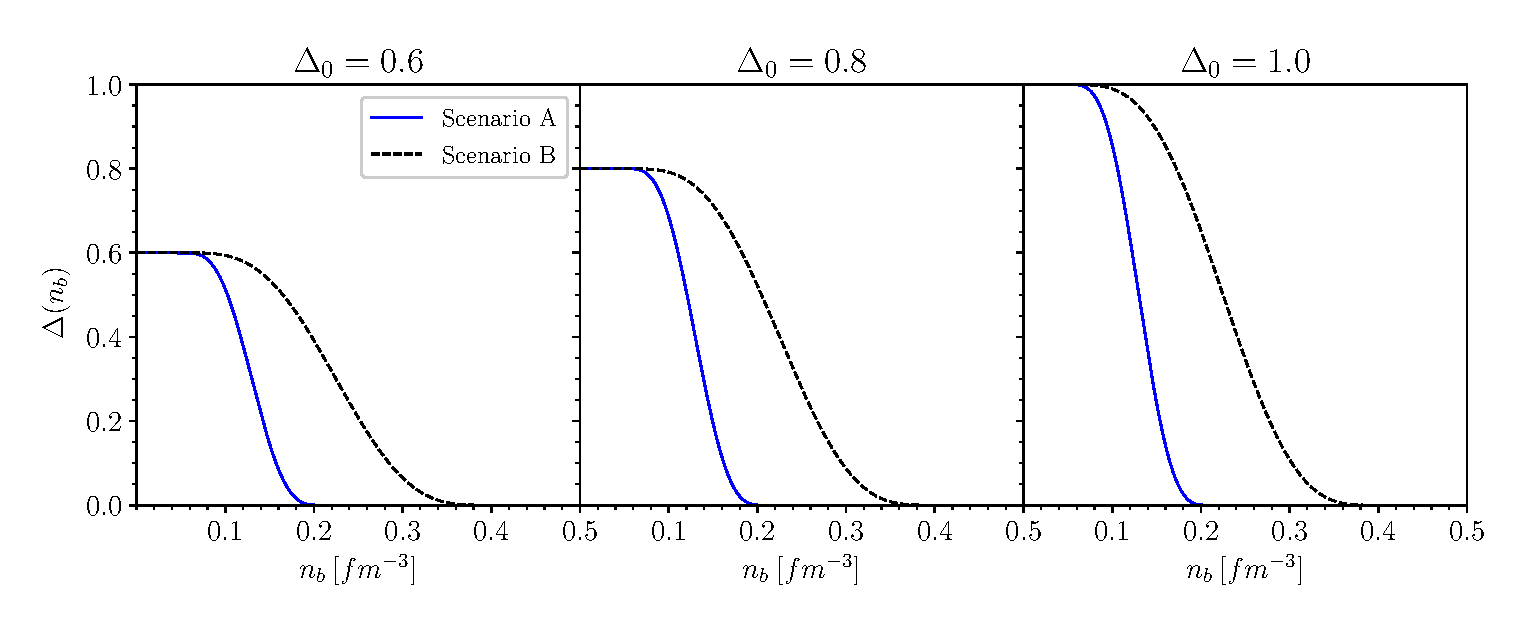
\includegraphics[width=\textwidth]{fig/Delta.eps}
    \caption{Different scenarios of the density dependence of the spin polarization 
		of baryons.}
    \label{fig:Delta}
\end{figure} 
\begin{figure}[ht!]
        \centering
        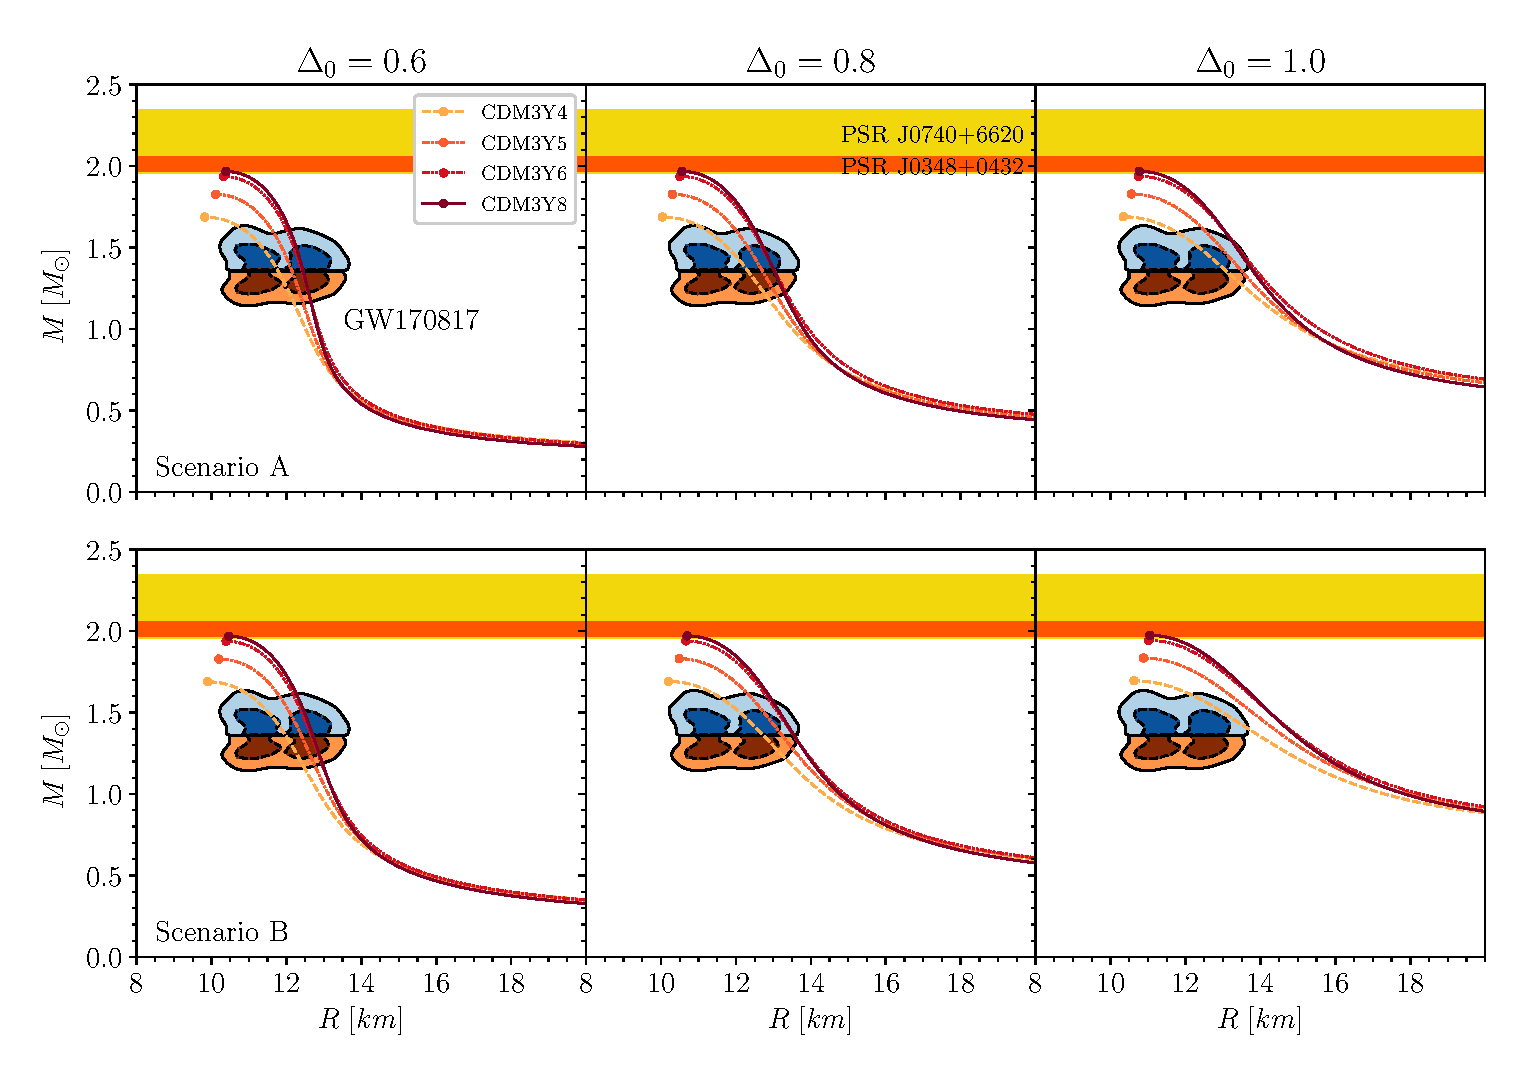
\includegraphics[width=\textwidth]{fig/MR.eps}
        \caption{The correlation of the gravitational mass $M$ and radius $R$ of magnetar 
            given by the solutions of the \gls{TOV} equations (\ref{tov}) obtained with different 
            EoS's of spin-polarized \gls{NS} matter. The empirical constraints for \gls{NS} with 
				mass of $1.4M_\odot$ inferred from the GW170817 data are shown by the colored contour,
				where the blue (red) shaded area represents the heavier (lighter) \gls{NS} 
				\citep{abbott2018gw170817}. The dot in each line indicates the maximum \gls{NS} 
				mass given by the corresponding EoS. The dark and light orange regions are the observed
				mass of the second \gls{PSR} J0348+0432 \citep{antoniadis2013massive} and 
				millisecond \gls{PSR} J0740+6620 \citep{cromartie2020relativistic} respectively.}
        \label{fig:mr}
\end{figure} 
Each scenario is assumed to have a starting value of the spin polarization of baryons 
at low densities, $\Delta_0 = 0.6$, $0.8$ and 1 as shown in Figure \ref{fig:Delta}.
The EoS's of $\beta$-stable $npe\mu$ matter obtained with different spin polarizations of 
baryons have been used as input for the \gls{TOV} equations (\ref{tov}), and the results obtained 
for the mass and radius of magnetar are shown in Figure \ref{fig:mr}. For comparison, we
have plotted in this Figure also the empirical constraint for the mass and radius of \gls{NS} 
around $M\approx 1.4 M_\odot$ implied by the tidal deformability of \gls{NS} estimated from 
the \gls{GW} signals of GW170817 \citep{abbott2018gw170817} (see more details on the tidal 
deformation of \gls{NS} in Sect.~\ref{sec3.2}), and the empirical mass limit of the second 
\gls{PSR} J0348+0432 ($M\approx 2.01^{+0.04}_{-0.04}M_\odot$) and millisecond 
\gls{PSR} J0740+6620 ($M\approx 2.14^{+0.20}_{-0.18}M_\odot$), the heaviest \glsplural{NS} 
observed so far. While the $M-R$ results given by 4 versions of the EoS with partial spin
polarizations of baryons ($\Delta_0 = 0.6\sim 0.8$) are within the empirical 
GW170817 constraint for \gls{NS} with $M=1.4M_\odot$, the \gls{NS} configurations starting with 
$\Delta_0 = 1.0$ seem to be out of the empirical range, as concluded recently 
by \cite{tan2020spin} and \cite{tews2020spin}. The radius of \gls{NS} with a 
$M\approx 1.4M_\odot$ obtained in scenario A with partial spin polarization 
of $\Delta_0 = 0.6$ is $R_{1/4}\approx 11.2 - 12.7$ km, which agrees well
with the empirical value $R_{1.4} \approx 11.75^{+0.86}_{-0.81}$ km deduced from 
the joint analysis of two \gls{NS} mergers GW170817 and GW190425 \citep{dietrich2020multimessenger}.
The spin polarization of baryons significantly enlarges the radius but affects minorly 
the mass of \gls{NS} as noted by \cite{tan2020spin}. In addition, the observed masses of two 
heaviest pulsars \gls{PSR} J0348+0432 and \gls{PSR} J0740+6620 allow us to trace the impact 
of the nuclear incompressibility $K$ on the \gls{NS} mass. Among four versions of the in-medium 
NN interaction used in the present HF calculation of NM, only the CDM3Y6 
and CDM3Y8 interactions (associated with $K\approx 252$ and 257 MeV) give the maximum 
gravitational mass of \gls{NS} close to the lower mass limit of the two heavy pulsars. These 
$K$ values are slightly higher than that around 240 MeV inferred from the structure studies 
of giant monopole resonances of finite nuclei \cite{garg2018compression}. In this connection we note 
a recent model-independent systematics of the astrophysical observations and results of the
ab-initio calculations by Annala et al. \cite{annala2020evidence}, which shows that the \gls{NS} 
matter in the interior of massive \gls{NS} with $M\approx 2M_\odot$ seems to contain deconfined 
baryons which form a quark-matter core in the center of \gls{NS}. Such a quark core can stiffen 
the EoS at highest densities of \gls{NS} matter and contributes up to 0.25 $M_\odot$ to the 
total \gls{NS} mass  \cite{annala2020evidence}. Therefore, a slight increase of the $K$ value given 
by the CDM3Y6 and CDM3Y8 interactions from the adopted value might be explained 
by a possible existence of the quark core in the center of heavy \gls{NS}.  

\subsection{Gravito-electric and gravito-magnetic deformability}%
\label{sec3.2}
In this chapter we address an interesting analogy between gravitation and electromagnetism
which has a long story because of similarity between Newton law for gravitational 
force and Coulomb law for electrostatic force \cite{mashhoon2003gravitoelectromagnetism}.
Here we discuss briefly the basic elements of gravitoelectromagnetism (\gls{GEM}) as 
presented by \cite{damour2009relativistic}. Assuming the linear perturbation of spacetime
by gravitation, the global inertial frame with $x^{\mu} = (ct, \mathbf{x})$ and 
Minkowski metric $\eta_{\mu\nu}$ can be expressed as
\begin{equation}
    g_{\mu\nu} \approx \eta_{\mu\nu} + h_{\mu\nu}(x),
\end{equation}
and the Einstein's field equations \eqref{Ein} reads
\begin{equation}
  \square \bar{h}_{\mu\nu} = - \frac{16\pi G}{c^4} T_{\mu\nu} \label{Ein_pert}
\end{equation}
where $\bar{h}_{\mu\nu}=h_{\mu\nu}-\frac{1}{2}\eta_{\mu\nu}\eta^{\rho\sigma}h_{\rho\sigma}$. Remarkably, the representation \eqref{Ein_pert} of the Einstein's field equation is 
completely analogous to the well-known Maxwell's equations of classical electromagnetism
\begin{equation}
    \square A^\nu = 4\pi J^\nu
\end{equation}
with $A$ being the electromagnetic field strength tensor and $J$ being the current 
4-vector. By introducing the \gls{GEM} potentials $\Phi$ and $\mathbf{A}$ via 
$\bar{h}_{00}=4\Phi/c^2$ and $\bar{h}_{0i} = -2A_i/c^2$, we define the \gls{GEM} fields as
\begin{equation}
E_{i} = -\partial_i\Phi - \frac{1}{2c}\pdv{A_i}{t},\ {\rm and}\ 
B_i = \epsilon_{ijk}\partial_j A_k,\ i,j,k=1,2,3. \label{eq3.9}
\end{equation}
Note that in the above evaluation, the background spacetime is supposed to be flat, 
in which the flat Minkowski metric was used. However, in a binary system of two \glsplural{NS}, 
the background metric around one \gls{NS} should be that of itself in isolation 
\citep{damour2009relativistic}, i.e., 
\begin{equation}
    G_{\mu\nu} = G^{(0)}_{\mu\nu} + H^{(1)}_{\mu\nu} + \ldots, \label{eq3.10} 
\end{equation}
where $G^{(0)}_{\mu\nu}$ is the metric of spacetime in the vicinity of an isolated \gls{NS} 
and $H^{(1)}_{\mu\nu}$ is the perturbation caused by its companion of the binary system. 
Following \cite{damour2009relativistic}, the perturbed metric takes the form 
\begin{equation}
    G_{00} = -\exp(-2W/c^2) \quad {\rm and}\quad G_{0a} = - \frac{4}{c^3} W_a \quad \text{with}\quad a=1,2,3.
		\label{eq3.11}
\end{equation}
The \emph{gravito-electric} (\gls{GE}) and \emph{gravito-magnetic} (\gls{GM}) fields 
in this case are defined in terms of post-Newtonian metric potential $W$ as
\begin{equation}
    E_a = \partial_a W + \frac{4}{c^2} \partial_t W_a,\quad {\rm and}\quad  
    B_a = \epsilon_{abc}\partial_b(-4W_c) \quad\text{with}\quad a,b,c=1,2,3. \label{eq3.12}
\end{equation}
Here the metric potential $W$ is determined in the local frame of the considered
NS. The \gls{GE} potential can then be reduced, in the nonrelativistic limit to 
Newtonian gravitation, to the classical gravitational potential $\sim GM/r$. 
By splitting the local metric potential $W$ into the \emph{internally-generated} and
\emph{externally-generated} parts, the GE and GM fields (\ref{eq3.12}) can be also
determined in terms of the corresponding internally- and externally-generated 
components. In the binary system of two merging NS, each NS companion feels
the tidal force of the gravitation field between them and becomes tidally deformed
in the local spacetime. It is natural that such tidal deformation of \gls{NS} 
is directly proportional to the strength of externally-generated parts of the GE 
and GM fields. The \emph{gravito-electric} and \emph{gravito-magnetic} relativistic tidal
moments of NS in the binary system are thus determined \citep{damour2009relativistic} as 
\begin{equation}
  G_L=\partial_{L-1} \bar{E}_{a_\ell} \qquad\text{and}\qquad 
	H_L = \partial_{L-1} \bar{B}_{a_\ell}, \label{eq3.13}
\end{equation}
where $\bar{E}_{a_\ell}$ and $\bar{B}_{a_\ell}$ are the $a_\ell$ components of the 
externally-generated local \gls{GE} and \gls{GM} fields, respectively. 
$L$ represents the multi-index $(a_1, a_2,\ldots, a_\ell)$, with $\ell$ being 
the order of the multipole moment. The GE and GM tidal multipole moments 
of NS are determined from the relativistic tidal moments (\ref{eq3.13}) through 
the coefficients $\lambda_\ell$ and $\sigma_\ell$, respectively.
\begin{equation}
    M_L=\lambda_\ell G_L \qquad {\rm and}\qquad S_L=\sigma_\ell H_L. \label{eq3.14}
\end{equation}
Here $M_L$ is the tidal mass multipole moment (associated with the deviation of the NS
mass distribution from the spherical shape at multipole $\ell$), and $S_L$ is the 
tidal current multipole moment \citep{damour2009relativistic,perot2021role}. 

The equations \eqref{eq3.14} give a direct link between the tidal field strengths 
and the tidal multipole moments of NS. The higher $\lambda_\ell$ (or $\sigma_\ell$) 
the stronger the \gls{NS} deforms under the same GE and GM tidal fields. From these
tidal multipole moments, the dimensionless \gls{GE} and \gls{GM} \emph{tidal Love numbers} 
are defined \citep{perot2021role} as 
\begin{equation}
k_\ell = \frac{1}{2} (2\ell-1)!! \frac{G\lambda_\ell}{R^{2\ell+1}} \quad \text{and}\quad 
j_\ell = 4(2\ell-1)!! \frac{G\sigma_\ell}{R^{2\ell+1}} 
\end{equation}
These parameters are directly related to the \gls{GE} and \gls{GM} 
\emph{tidal deformability parameters} as
\begin{IEEEeqnarray}{rCl}
    \Lambda_\ell &=& \frac{2}{(2\ell-1)!!} k_\ell \left(\frac{c^2 R}{GM} \right)^{2\ell+1}, 
		\label{eq:Lambda}\\
    \Sigma_\ell &=& \frac{1}{4(2\ell-1)!!} j_\ell \left( \frac{c^2 R}{GM} \right)^{2\ell+1}.
\end{IEEEeqnarray}
The observed  GW signals of the NS merger GW170817 have been analyzed to infer the
constraint for the $\Lambda_2$ component of the tidal deformability which was then 
translated into the constraint for the gravitational mass and radius of NS shown 
in Fig.~\ref{fig:mr}. 

In the present work we perform the explicit calculation of the tidal deformability 
parameters. With $H_\ell(r)$ and $\tilde{H}_\ell(r)$ characterizing small even and
odd-parity perturbations on the static metric, which in turn relate directly to
the \gls{GE} and \gls{GM} tidal moment \eqref{eq3.13} after matching the
``internal'' and ``external'' problems as proceded by \cite{damour2009relativistic},
the two ``master equations'' governing these two types of perturbations in the
\gls{NS}'s interior are 
\citep{perot2021role}
\begin{IEEEeqnarray*}{rCl}
        H''_\ell(r) &+& H'_\ell(r) \left[ 1-\frac{2Gm(r)}{c^2 r}  \right]^{-1} \left\{ \frac{2}{r} - \frac{2Gm(r)}{c^2 r^2} - \frac{4\pi G}{c^4} r[\rho(r)c^2 - P(r)] \right\}\\
                 &+& H_\ell(r) \left[ 1-\frac{2Gm(r)}{c^2 r} \right]^{-1} \Bigg\{ \frac{4\pi G}{c^4} \left[ 5\rho(r)c^2 + 9P(r) + c^2 \dv{\rho}{P}\left[ \rho(r)c^2 + P(r) \right] \right] \\
                 &-& \frac{\ell(\ell+1)}{r^2} - 4 \left[ 1-\frac{2Gm(r)}{c^2 r} \right]^{-1} \left[ \frac{Gm(r)}{c^2 r^2} + \frac{4\pi G}{c^4} rP(r) \right]^2 \Bigg\} = 0\IEEEyesnumber
\end{IEEEeqnarray*}
for \gls{GE} perturbations and
\begin{IEEEeqnarray*}{rCl}
        \tilde{H}''_\ell(r) &-& \tilde{H}'_\ell(r) \left[ 1-\frac{2Gm(r)}{c^2 r} \right]^{-1} \frac{4\pi G}{c^4} r \left[ P(r) + \rho(r)c^2 \right]\\
                         &-& \tilde{H}_\ell(r) \left[ 1-\frac{2Gm(r)}{c^2 r} \right]^{-1} \left\{ \frac{\ell(\ell+1)}{r^2} - \frac{4Gm(r)}{c^2 r^3} + \theta \frac{8\pi G}{c^4} \left[ P(r) + \rho(r)c^2 \right] \right\} = 0\\\IEEEyesnumber
\end{IEEEeqnarray*}
for \gls{GM} perturbations; the value of $\theta=1$ is for static fluid while irrotational fluid adopts the value $\theta=-1$. These equations govern the even and odd parity parts of the stationary perturbation of the background metric, as developed by \cite{damour2009relativistic}, and are integrated along with the \gls{TOV} equation \eqref{tov}. In addition, we have the compactness parameters $C = GM/(Rc^2)$ and define
\begin{equation}
        y_\ell = \frac{RH'_\ell(R)}{H_\ell(R)} \quad\text{and}\quad \tilde{y}_\ell = \frac{R\tilde{H}'_\ell(R)}{\tilde{H}_\ell(R)}.
\end{equation}
The explicit expressions of the first few orders of the \gls{GE} and \gls{GM} Love numbers are 
{\allowdisplaybreaks
\begin{IEEEeqnarray*}{rCl}
        k_2 &=& \frac{8}{5} C^5 (1-2C)^2 \left[ 2(y_2 -1)C - y_2 + 2 \right] \left\{ 2C \left[ 4(y_2 +1)C^4 + 2(3y_2 -2)C^3\right.\right.\\
            && \negmedspace{}\left. -2(11y_2 -13)C^2 + 3(5y_2 -8)C - 3(y_2 -2) \right]\\
            && \negmedspace{}\left. +3(1-2C)^2 \left[ 2(y_2 -1)C - y_2 +2 \right]\log (1-2C) \right\}^{-1},\IEEEyesnumber\\
        k_3 &=& \frac{8}{7} C^7 (1-2C)^2 \left[ 2(y_3 - 1)C^2 - 3(y_3 -2)C + y_3 -3 \right] \times \left\{2C \big[ 4(y_3 + 1)C^5 \right.\\
            &&\negmedspace{} \times + 2(9y_3 -2)C^4 - 20(7y_3 -9)C^3 + 5(37y_3 -72)C^2 - 45(2y_3 -5)C + 15(y_3 - 3)\big]\\
            &&\negmedspace{}\left. + 15(1-2C)^2 \left[ 2(y_3 -1)C^2 - 3(y_3 -2)C + y_3 - 3 \right]\log (1-2C)\right\}^{-1},\IEEEyesnumber\\
        k_4 &=& \frac{32}{147} C^9 (1-2C)^2 \left[ 12(y_4 -1)C^3 - 34(y_4 -2)C^2 + 28(y_4 -3)C -7(y_4 -4) \right]\\
            &&\negmedspace{} \times \left\{ 2C \left[ 8(y_4 +1)C^6 + 4(17y_4 -2)C^5 - 12(83y_4 -107)C^4 + 40(55y_4 -116)C^3 \right.\right.\\
            &&\negmedspace{} \left.\left. - 10(191y_4 -536)C^2 + 105(7y_4 -24)C - 105(y_4 -4)\right] + 15(1-2C)^2 \left[ 12(y_4 -1)C^3\right.\right.\\
            &&\negmedspace{} \left.\left. -34(y_4 -2)C^2 + 28(y_4 -3)C - 7(y_4 -4)\right]\log (1-2C)\right\}^{-1},\IEEEyesnumber\\
        j_2 &=& \frac{24}{5} C^5 \left[ 2(\tilde{y}_2 -2)C - \tilde{y}_2 +3 \right] \big\{ 2C \left[ 2(\tilde{y}_2 +1)C^3 + 2\tilde{y}_2 C^2 + 3(\tilde{y}_2 -1)C - 3(\tilde{y}_2 -3) \right]\\
            &&\negmedspace{} +3 \left[ 2(\tilde{y}_2 -2)C - \tilde{y}_2 +3 \right]\log (1-2C)\big\}^{-1},\IEEEyesnumber\\
        j_3 &=& \frac{64}{21} C^7 \left[ 8(\tilde{y}_3 -2)C^2 - 10(\tilde{y}_3 -3)C + 3(\tilde{y}_3 -4) \right]\\
            &&\negmedspace{} \times \left\{ 2C \left[ 4(\tilde{y}_3 +1)C^4 + 10\tilde{y}_3 C^3 + 30(\tilde{y}_3-1)C^2 - 15(7\tilde{y}_3 -18)C + 45(\tilde{y}_3 -4) \right]\right.\\
            &&\negmedspace{} \left. + 15 \left[ 8(\tilde{y}_3 -2)C^2 - 10(\tilde{y}_3 -3)C + 3(\tilde{y}_3 -4) \right]\log(1-2C) \right\}^{-1},\IEEEyesnumber\\
        j_4 &=& \frac{80}{147} C^9 \left[ 40(\tilde{y}_4 -2)C^3 - 90(\tilde{y}_4 -3)C^2 + 63(\tilde{y}_4 -4)C - 14(\tilde{y}_4 -5) \right]\\
            &&\negmedspace{} \times \left\{ 2C \big[ 4(\tilde{y}_4 +1)C^5 + 18\tilde{y}_4 C^4 + 90(\tilde{y}_4 -1)C^3 - 5(137\tilde{y}_4 -334)C^2\right.\\
            &&\negmedspace{} \left. + 105(7\tilde{y}_4 -26)C - 210(\tilde{y}_4 -5)\big] + 15 \big[ 40(\tilde{y}_4 -2)C^3 - 90(\tilde{y}_4 -3)C^2\right.\\
            &&\negmedspace{} \left. + 63(\tilde{y}_4 -4)C - 14(\tilde{y}_4 -5) \big]\log(1-2C)\right\}^{-1} \IEEEyesnumber
\end{IEEEeqnarray*}
}
as derived by \cite{perot2021role}.

\begin{figure}[ht!]
        \centering
        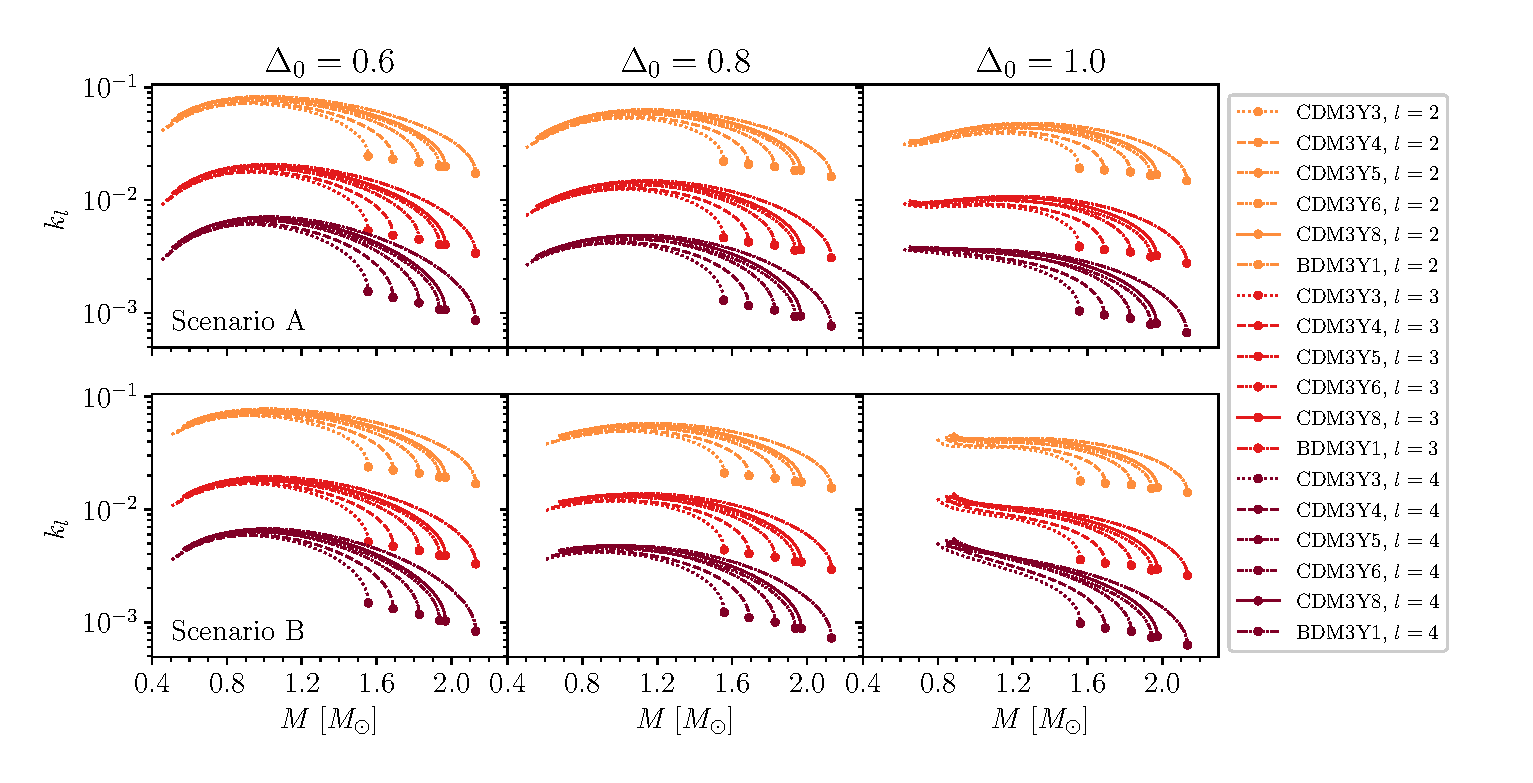
\includegraphics[width=\textwidth]{fig/kl.eps}
        \caption{\gls{GE} tidal Love number at $\ell$\textsuperscript{th} order $k_\ell$ as function of magnetar mass computed with 4 density-dependent \gls{NN} interaction versions at different spin polarizations. The dot at the end of each line represents the maximum gravitational mass $M$ of the magnetar generated by the corresponding \gls{EoS}.}
        \label{fig:kl}
\end{figure} 
\begin{figure}[ht!]
    \centering
    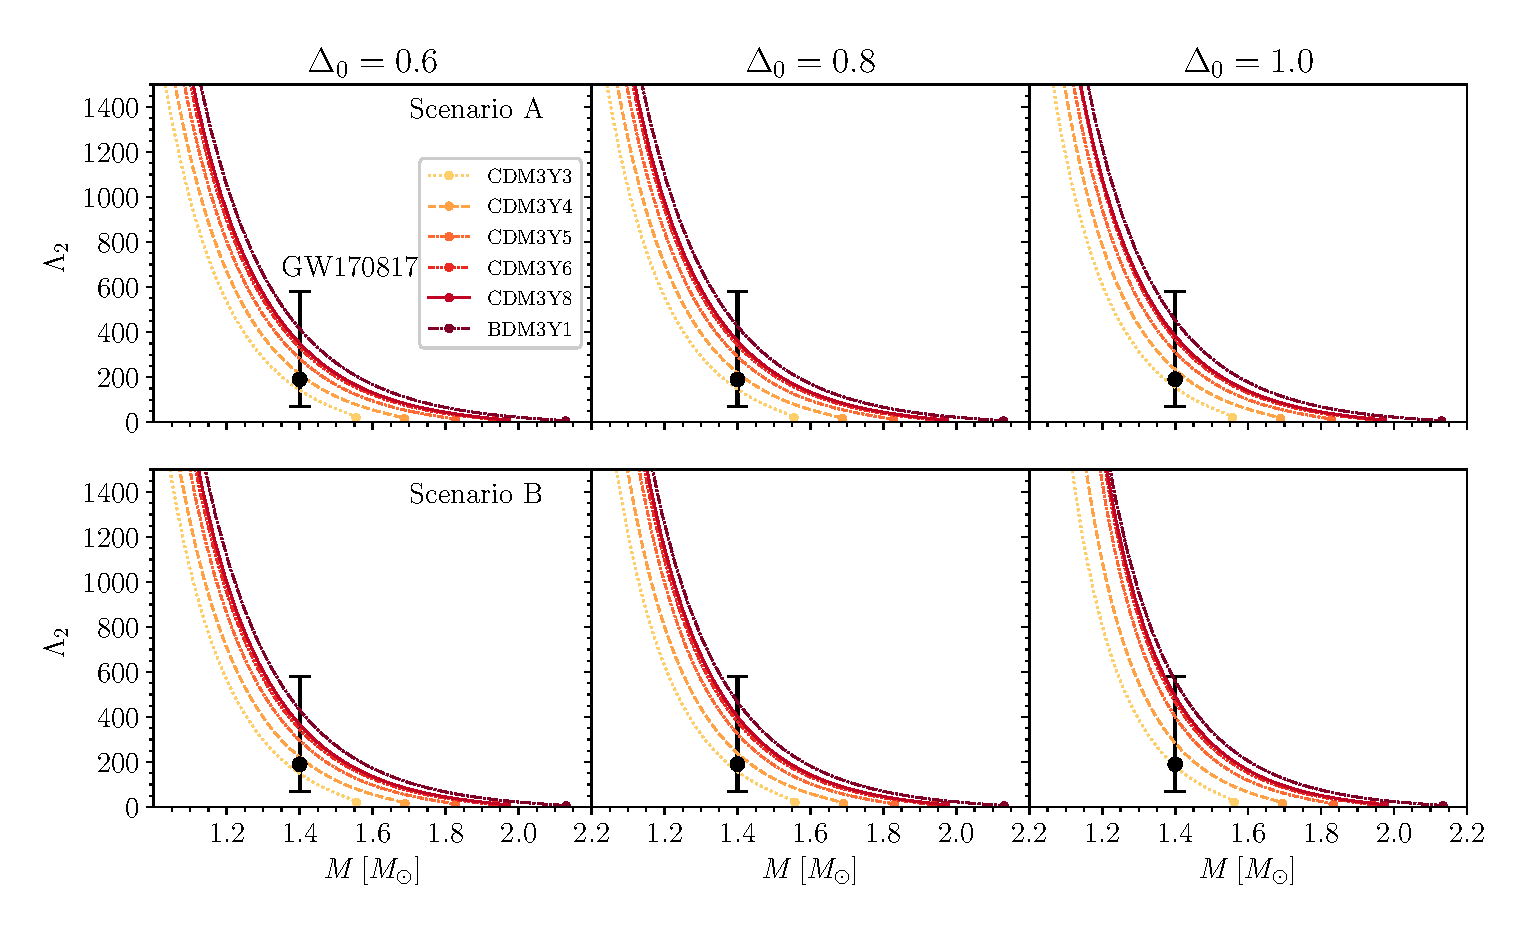
\includegraphics[width=\textwidth]{fig/Lambda2.eps}
    \caption{Dimensionless \gls{GE} tidal deformability parameter of 2\textsuperscript{nd} order $\Lambda_2$ of different CDM3Y$n$ models with varying $\Delta$. The vertical bar is the empirical tidal deformability constraint $\Lambda_2 \approx 190_{-120}^{+390}$ at $1.4M_\odot$, obtained from the Bayesian analysis of GW170817 data with 90\% confidence level \citep{abbott2018gw170817}.}
    \label{fig:Lambda2}
\end{figure} 
The results for \gls{GE} tidal Love number's dependence on \gls{NS}'s gravitational mass arose from 4 versions of the \gls{EoS} are shown in Figure \ref{fig:kl}. Similar to \cite{perot2021role}, in this result, it is clear that the higher the order $\ell$, the less impactful the Love number $k_\ell$ is for the tidal properties of the \gls{NS}, i.e. $k_\ell$ tends to be smaller by an order of magnitude than $k_{\ell-1}$, as expected from the multipole expansion. The 2\textsuperscript{nd} order is consequently dominant compared to the others. Between two scenarios A and B, at partial polarization of $\Delta_0 = 0.6$, the difference in $k_\ell$ of the same order is insignificant, except for the small difference in the low mass section. On the other hand, for the case of higher spin polarity in the \gls{NS} surface, the results are much more distinguishable, as the computation with scenario B gives rise to a ``steeper'' curve of $k_\ell$. Furthermore, in general, the maximum values of $k_\ell$ are at the common gravitational mass $M$ at all orders computed so far, and this value of $M$ seems to only depends on the value of $\Delta_0$, where the position of maximum $k_\ell$ tends to be shifted to a higher $M$ as $\Delta_0$ increases. Among these tidal parameters, the only one that has been constrained by far is the dominant 2\textsuperscript{nd} order Love number, which is investigated through the closely related dimensionless tidal deformability parameter of second order $\Lambda_2$ \eqref{eq:Lambda} and whose results are given in Figure \ref{fig:Lambda2}. In the study of \cite{abbott2018gw170817}, the range of $\Lambda_2$ is accepted to be $\Lambda_2 \approx 190^{+390}_{-120}$ at $M=1.4M_\odot$. It is interesting to note that for all cases in this study, this constraint tolerates all \glsplural{EoS} and scenarios, as well as the value of $\Delta_0$, thus no further exclusion can be done with this parameter. It's worth mentioning that the nuclear incompressibility $K$ plays a significant role in determining the tidal deformability $\Lambda_2$ as when $K$ varies from version to version (CDM3Y4 to CDM3Y8), the value of $\Lambda_2$ increases by $\approx 3$ times for the scenario A of $\Delta_0 = 0.6$ case, the same can be said for the different configuration of $\Delta(n_b)$. Testing the values of $k_\ell$ at higher orders can also be done by evaluating the tidal correction of the \gls{GW} waveform from inspiralling \glsplural{NS} within the PN theory, i.e. the \gls{GE} contribution of order $(2\ell+1)$PN to the phase of \gls{GW} signal is \citep{perot2021role, yagi2014multipole}
\begin{equation}
    \Psi_\ell = - \sum^{2}_{i=1} \left[ \frac{5}{16} \frac{(2\ell-1)!! (4\ell+3)(\ell+1)}{(4\ell-3)(2\ell-3)} \Lambda_{\ell,i} X_i^{2\ell-1} x^{2\ell - 3/2} + \frac{9}{16} \delta_{\ell 2} \Lambda_{2, i} \frac{X_i^4}{\eta} x^{5/2} \right] + \mathcal{O}(x^{2\ell-1/2})
\end{equation}
where $i=1,\,2$ is the index distinguishing the two \glsplural{NS} of the system, $x=\left( G\pi Mf/c^3 \right)^{2/3}$, $f$ is the \gls{GW} signal frequency, $M=M_1 + M_2$, $X_i = M_i/M$ and $\eta = M_1 M_2/M^2$.

The gravito-magnetic tidal Love numbers $j_\ell$ contribute more weakly to the \gls{GW} phase compared to that of their \gls{GE} counterpart, as the \gls{GM} terms only appear from higher orders of $(2\ell+2)$PN, where the first correction at 6PN is given by \citep{perot2021role,yagi2017erratum}
\begin{equation}
    \tilde{\Psi}_2 = \sum^{2}_{i=1} \frac{5}{224} \sigma_{2,i} \frac{X_i^4}{\eta} \left( X_i - 1037X_j \right)x^{7/2} + \mathcal{O}(x^{9/2})
\end{equation}
\begin{figure}[ht!]
        \centering
        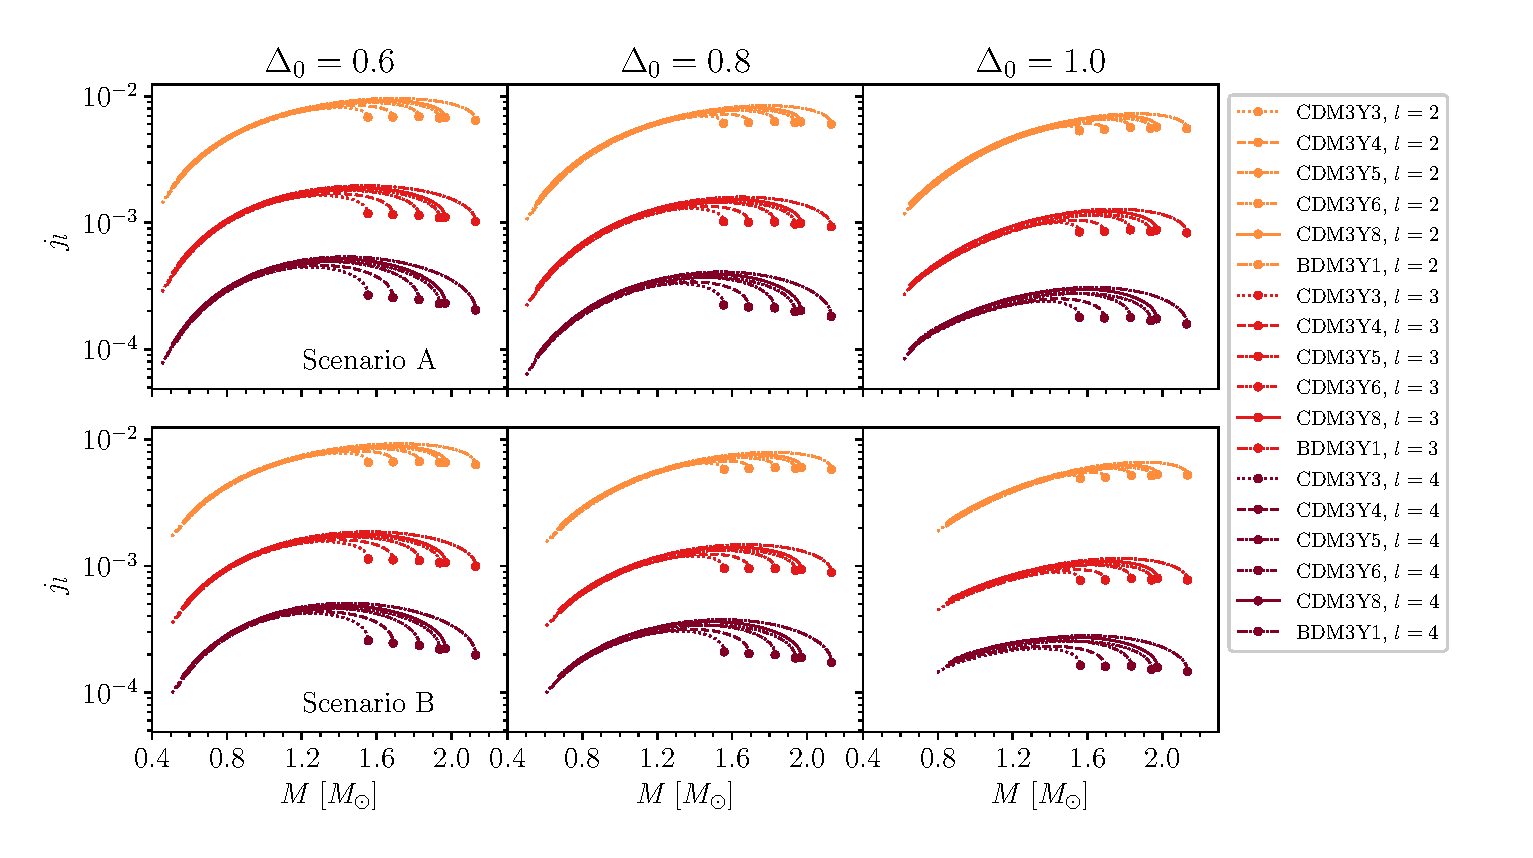
\includegraphics[width=\textwidth]{fig/jl_stat.eps}
        \caption{\gls{GM} tidal Love number at $\ell$\textsuperscript{th} order $j_\ell$ as function of \gls{NS} mass computed with CDM3Y$n$ models of \emph{strictly static fluid} at different polarizations.}
        \label{fig:jl_stat}
\end{figure} 
\begin{figure}[ht!]
        \centering
        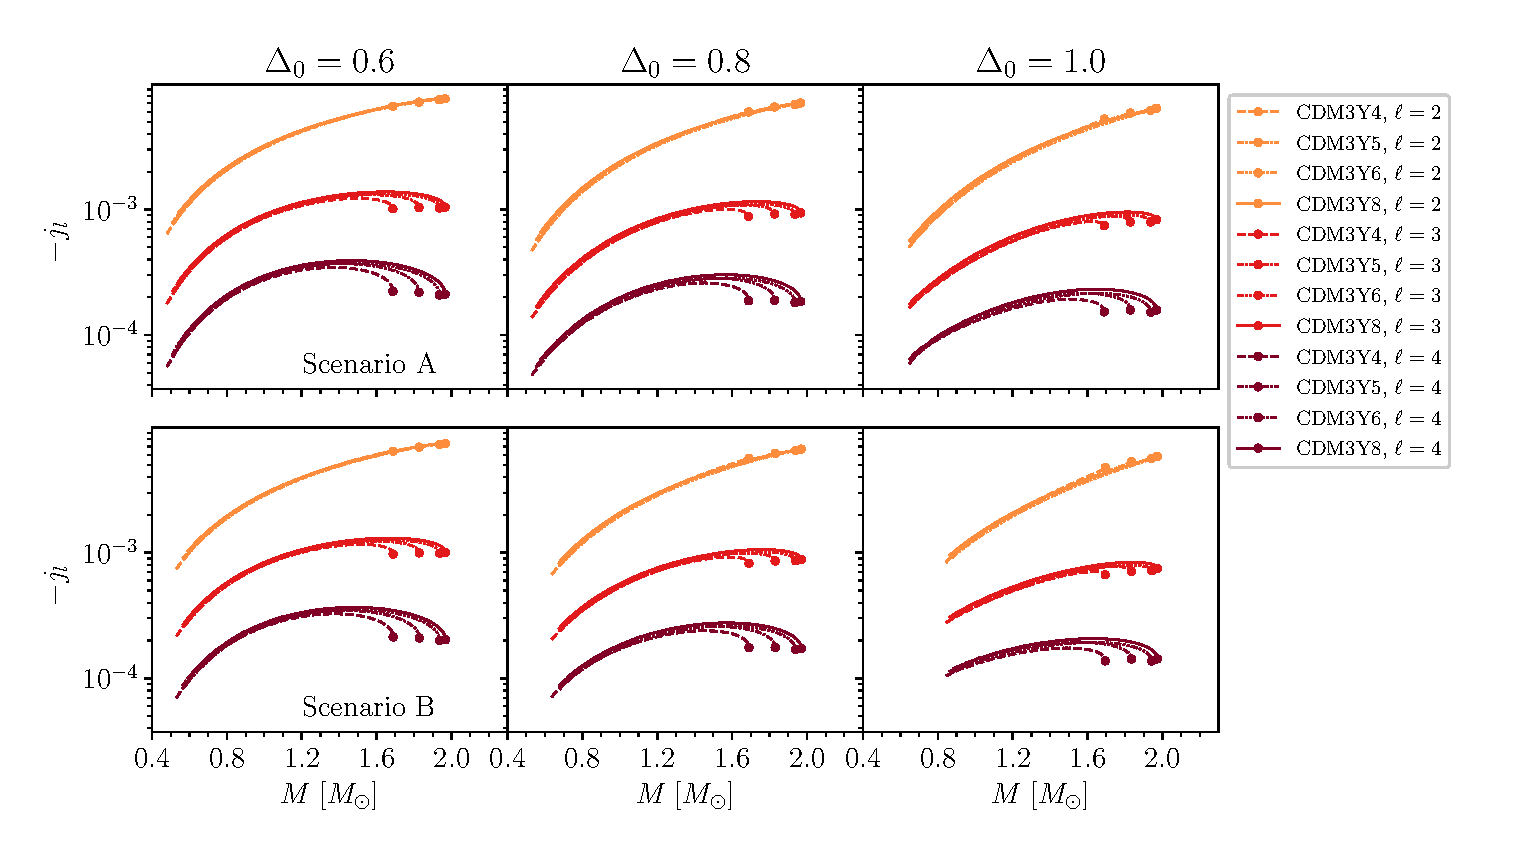
\includegraphics[width=\textwidth]{fig/jl_irrot.eps}
        \caption{\gls{GM} tidal Love number at $\ell$\textsuperscript{th} order $j_\ell$ as function of \gls{NS} mass computed with CDM3Y$n$ models of \emph{irrotational fluid} at different polarizations.}
        \label{fig:jl_irrot}
\end{figure} 
The \gls{GM} tidal Love numbers of second, third and fourth order computed with 4 different \glsplural{EoS} are shown in Figure \ref{fig:jl_stat} for strictly static fluid and \ref{fig:jl_irrot} for irrotational fluid. Apart from the same trends as the \gls{GE} tidal Love numbers discussed previously, the \gls{GM} Love numbers' values do not have much variation as $\Delta_0$ increases in each scenario, as the shape of each curves in Figure \ref{fig:jl_stat} doesn't differ far from each others except for the difference in range of gravitational mass $M$. The value of $j_\ell$ corresponding to the \gls{GM} pertubation of irrotational fluid (Figure \ref{fig:jl_irrot}), on the other hand, stands out from the other two types of Love numbers, where its value is completely negative, albeit having the same magnitude as that of static fluid, this type of fluid motion is stated to be more realistic in this case due to it being driven by the tides \citep{perot2021role,pani2018magnetic}. In this case, the lines traced by each interation appear to reach maximum value at the maximum $M$ at the leading terms only, rather than having a local maxima in between. The dominance of the 2\textsuperscript{nd} order terms are clear in all cases, where the difference of around one order of magnitude is maintained. Notably, for the \gls{GM} terms corresponding with each \gls{NN} interaction, at higher order $\ell$, the \gls{NS} mass at maximum $j_\ell$ seems to become smaller. One more interesting result is that the magnitudes of $j_\ell$ for two types of fluid are also comparable but is smaller than their \gls{GE} counterpart by one order of magnitude, similar to the conclusion reached by \cite{perot2021role}.
